%%%%%%%%%%%%%%%%%%%%%%%%%%%%%%%%%%%%%%%%%
% Nat64 support for IML
% Module cpib
%
% This template was downloaded from:
% http://www.LaTeXTemplates.com
%
% Authors:
% Marco Romanutti
% Benjamin Meyer
%
% License:
% CC BY-NC-SA 3.0 (http://creativecommons.org/licenses/by-nc-sa/3.0/)
%
%%%%%%%%%%%%%%%%%%%%%%%%%%%%%%%%%%%%%%%%%

%----------------------------------------------------------------------------------------
%	PACKAGES AND OTHER DOCUMENT CONFIGURATIONS
%----------------------------------------------------------------------------------------

\documentclass[10pt, a4paper, twocolumn]{article} % 10pt font size (11 and 12 also possible), A4 paper (letterpaper for US letter) and two column layout (remove for one column)

%%%%%%%%%%%%%%%%%%%%%%%%%%%%%%%%%%%%%%%%%
% Bloom filter
% Module dist
% Assignment 02
%
% This template was downloaded from:
% http://www.LaTeXTemplates.com
%
% Authors:
% Marco Romanutti
% Dominik Fringeli
%
% License:
% CC BY-NC-SA 3.0 (http://creativecommons.org/licenses/by-nc-sa/3.0/)
%
%%%%%%%%%%%%%%%%%%%%%%%%%%%%%%%%%%%%%%%%%

%----------------------------------------------------------------------------------------
%	PACKAGES AND OTHER DOCUMENT CONFIGURATIONS
%----------------------------------------------------------------------------------------

\usepackage[english]{babel} % English language hyphenation

\usepackage{microtype} % Better typography

\usepackage{amsmath,amsfonts,amsthm} % Math packages for equations

\usepackage[svgnames]{xcolor} % Enabling colors by their 'svgnames'

\usepackage[hang, small, labelfont=bf, up, textfont=it]{caption} % Custom captions under/above tables and figures

\usepackage{booktabs} % Horizontal rules in tables

\usepackage{lastpage} % Used to determine the number of pages in the document (for "Page X of Total")

\usepackage{graphicx} % Required for adding images
\usepackage{float} % Force image placement

\usepackage{enumitem} % Required for customising lists
\setlist{noitemsep} % Remove spacing between bullet/numbered list elements

\usepackage{sectsty} % Enables custom section titles

\usepackage{tabularx} % Pro/cons table
\allsectionsfont{\usefont{OT1}{phv}{b}{n}} % Change the font of all section commands (Helvetica)

\usepackage{ marvosym } % Symbols
%----------------------------------------------------------------------------------------
%	MARGINS AND SPACING
%----------------------------------------------------------------------------------------

\usepackage{geometry} % Required for adjusting page dimensions

\geometry{
	top=1cm, % Top margin
	bottom=1.5cm, % Bottom margin
	left=2cm, % Left margin
	right=2cm, % Right margin
	includehead, % Include space for a header
	includefoot, % Include space for a footer
	%showframe, % Uncomment to show how the type block is set on the page
}

\setlength{\columnsep}{7mm} % Column separation width

%----------------------------------------------------------------------------------------
%	FONTS
%----------------------------------------------------------------------------------------

\usepackage[T1]{fontenc} % Output font encoding for international characters
\usepackage[utf8]{inputenc} % Required for inputting international characters

\usepackage{XCharter} % Use the XCharter font

\usepackage{amssymb}% http://ctan.org/pkg/amssymb
\usepackage{pifont}% http://ctan.org/pkg/pifont
\newcommand{\cmark}{\ding{51}}%
\newcommand{\xmark}{\ding{55}}%

%----------------------------------------------------------------------------------------
%	HEADERS AND FOOTERS
%----------------------------------------------------------------------------------------

\usepackage{fancyhdr} % Needed to define custom headers/footers
\pagestyle{fancy} % Enables the custom headers/footers

\renewcommand{\headrulewidth}{0.0pt} % No header rule
\renewcommand{\footrulewidth}{0.4pt} % Thin footer rule

\renewcommand{\sectionmark}[1]{\markboth{#1}{}} % Removes the section number from the header when \leftmark is used

%\nouppercase\leftmark % Add this to one of the lines below if you want a section title in the header/footer

% Headers
\lhead{} % Left header
\chead{\textit{\thetitle}} % Center header - currently printing the article title
\rhead{} % Right header

% Footers
\lfoot{} % Left footer
\cfoot{} % Center footer
\rfoot{\footnotesize Seite \thepage\ von \pageref{LastPage}} % Right footer, "Page 1 of 2"

\fancypagestyle{firstpage}{ % Page style for the first page with the title
	\fancyhf{}
	\renewcommand{\footrulewidth}{0pt} % Suppress footer rule
}

%----------------------------------------------------------------------------------------
%	TITLE SECTION
%----------------------------------------------------------------------------------------

\newcommand{\authorstyle}[1]{{\large\usefont{OT1}{phv}{b}{n}\color{DarkRed}#1}} % Authors style (Helvetica)

\newcommand{\institution}[1]{{\footnotesize\usefont{OT1}{phv}{m}{sl}\color{Black}#1}} % Institutions style (Helvetica)

\usepackage{titling} % Allows custom title configuration

\newcommand{\HorRule}{\color{DarkGoldenrod}\rule{\linewidth}{1pt}} % Defines the gold horizontal rule around the title

\pretitle{
	\vspace{0pt} % Move the entire title section up
	\HorRule\vspace{10pt} % Horizontal rule before the title
	\fontsize{32}{36}\usefont{OT1}{phv}{b}{n}\selectfont % Helvetica
	\color{DarkRed} % Text colour for the title and author(s)
}

\posttitle{\par\vskip 15pt} % Whitespace under the title

\preauthor{} % Anything that will appear before \author is printed

\postauthor{ % Anything that will appear after \author is printed
	\vspace{10pt} % Space before the rule
	\par\HorRule % Horizontal rule after the title
	\vspace{-34pt} % Space after the title section
}

%----------------------------------------------------------------------------------------
%	ABSTRACT
%----------------------------------------------------------------------------------------

\usepackage{lettrine} % Package to accentuate the first letter of the text (lettrine)
\usepackage{fix-cm}	% Fixes the height of the lettrine

\newcommand{\initial}[1]{ % Defines the command and style for the lettrine
	\lettrine[lines=3,findent=4pt,nindent=0pt]{% Lettrine takes up 3 lines, the text to the right of it is indented 4pt and further indenting of lines 2+ is stopped
		\color{DarkGoldenrod}% Lettrine colour
		{#1}% The letter
	}{}%
}

\usepackage{xstring} % Required for string manipulation

\newcommand{\lettrineabstract}[1]{
	\StrLeft{#1}{1}[\firstletter] % Capture the first letter of the abstract for the lettrine
	\initial{\firstletter}\textbf{\StrGobbleLeft{#1}{1}} % Print the abstract with the first letter as a lettrine and the rest in bold
}

%----------------------------------------------------------------------------------------
%	LISTINGS
%----------------------------------------------------------------------------------------

\usepackage{listings}
\usepackage{color}
\usepackage[listings]{tcolorbox}

\definecolor{dkgreen}{rgb}{0,0.6,0}
\definecolor{gray}{rgb}{0.5,0.5,0.5}
\definecolor{mauve}{rgb}{0.58,0,0.82}

\lstset{frame=tb,
language=Java,
aboveskip=3mm,
belowskip=3mm,
showstringspaces=false,
columns=flexible,
basicstyle={\small\ttfamily},
numbers=none,
numberstyle=\tiny\color{gray},
keywordstyle=\color{blue},
commentstyle=\color{dkgreen},
stringstyle=\color{mauve},
breaklines=true,
breakatwhitespace=true,
tabsize=3
}

%----------------------------------------------------------------------------------------
%	BIBLIOGRAPHY
%----------------------------------------------------------------------------------------

\usepackage[backend=bibtex,style=authoryear,natbib=true]{biblatex} % Use the bibtex backend with the authoryear citation style (which resembles APA)

\addbibresource{example.bib} % The filename of the bibliography

\usepackage[autostyle=true]{csquotes} % Required to generate language-dependent quotes in the bibliography
 % Specifies the document structure and loads requires packages

%----------------------------------------------------------------------------------------
%	ARTICLE INFORMATION
%----------------------------------------------------------------------------------------

\title{Nat64 und Casting für IML} % The article title

\author{
	\authorstyle{Marco Romanutti\textsuperscript{1,2} und Benjamin Meyer\textsuperscript{1,2}} % Authors
	\newline\newline % Space before institutions
	\textsuperscript{1}\institution{Fachhochschule Nordwestschweiz FHNW, Brugg}\\ % Institution
	\textsuperscript{2}\texttt{Zwischenbericht} % Module
}

\date{}

%----------------------------------------------------------------------------------------

\begin{document}

\maketitle % Print the title

\thispagestyle{firstpage} % Apply the page style for the first page (no headers and footers)

%----------------------------------------------------------------------------------------
%	ABSTRACT
%----------------------------------------------------------------------------------------

%\lettrineabstract{Im Modul Compilerbau soll eine Erweiterung für eine bestehende IML spezifiziert und implementiert werden. Unsere Erweiterung führt die Unterstützung eines Datentypen für natürliche Zahlen ein. In den nachfolgegenden Abschnitten werden die Erweiterungen an der IML-Spezifikation beschrieben und Implementationsentscheide begründet.}
%\lettrineabstract{Im Modul Compilerbau wird eine Erweiterung für die bestehende Sprache IML spezifiziert und implementiert. Neu soll ein Datentyp für natürliche Zahlen unterstützt werden. Werte vom bestehenden Datentyp int64 können in den neuen Datentypen gecastet werden und umgekehrt.}
\lettrineabstract{Im Modul Compilerbau wird eine Erweiterung für die bestehende Sprache IML spezifiziert und implementiert. Die Implementierung beinhaltet einen neuen Datentyp für natürliche Zahlen, sowie eine Möglichkeit den Datentyp int64 in den neuen Datentyp zu casten und umgekehrt.}
%----------------------------------------------------------------------------------------
%	ARTICLE CONTENTS
%----------------------------------------------------------------------------------------

\section{Compiler}
Der Compiler basiert auf der IML (V2) und ist in Java geschrieben.

\section{Erweiterung}
\subsection{Einleitung}
Unter natürlichen Zahlen werden die positiven, ganzen Zahlen und 0 verstanden.
Die IML soll um einen neuen Datentyp \texttt{nat64} erweitert werden.
Der neue Datentyp soll solche positiven, ganzen Zahlen mit bis Länge 64 in Binärdarstellung abbilden können.
Es sollen die bestehenden Operationen unterstützt werden.
Ausserdem soll ein explizites Casting zwischen dem bestehenden Datentyp \texttt{int64} und dem neuen Datentyp \texttt{nat64} möglich sein.

\subsection{Lexikalische Syntax}
Für den neuen Datentyp wird das Keyword \texttt{(TYPE, NAT64)} und ein Castingoperator hinzugefügt.

% Listing mit neuen Elementen
\begin{lstlisting}[backgroundcolor = \color{lightgray},
xleftmargin = 0.05cm,
framexleftmargin = 0.05em]
    Datentyp:     nat64     (TYPE, NAT64)
    Brackets:     [ ]       LBRACKET, RBRACKET
\end{lstlisting}

Casting ist nur von \texttt{(TYPE, INT64)} zu \texttt{(TYPE, NAT64)} und umgekehrt möglich.
Als Castingoperator wird die rechtekige Klammern (nachfolgend Brackets gennant) verwendet.
Innerhalb der Brakets befindet sich der Zieldatentyp \footnote{zum Beispiel \texttt{[int64]}}.

\subsection{Grammatikalische Syntax}
Das nachfolgende Code-Listing zeigt, wie der neue Datentyp \texttt{nat64} eingesetzt werden kann.
\begin{lstlisting}
// Deklaration
var natIdent1 : nat64;
var natIdent2 : nat64;
var natIdent3 : nat64;

// Initialisierung
natIdent1 init := 50;
natIdent2 init := 10;
natIdent3 init := natIdent1 + natIdent2;

// Casting von int64 nach nat64
var intIdent1 : int64;
intIdent1 init := 30;
natIdent3 := [nat64] intIdent1;

call functionWithNatParam([nat64] intIdent1);

// Casting von nat64 nach int64
var intIdent2 : int64;
intIdent2 init := [int64] natIdent3;

call functionWithIntParam([int64] natIdent3);
\end{lstlisting}
Falls zwei Datentypen nicht gecastet werden können, wird ein Kompilierungsfehler geworfen.
Folgendes Code-Listing zeigt ein solches Beispiel mit dem bestehenden Datentyp \texttt{bool}:
\begin{lstlisting}
// Deklaration
var boolIdent : bool;
boolIdent init := false;

var natIdent : nat64;
// Throws type checker error:
natIdent init := [nat64] boolIdent
\end{lstlisting}
Unsere Erweiterung unterstützt keine impliziten Castings.
Weitere Code-Beispiele sind in Kapitel \ref{sec:prog} zu finden.

\subsection{Änderungen an der Grammatik}

Zusätzlich zu den bestehende Operatoren wurde ein neuer \texttt{castOpr} erstellt, welcher anstelle des Nichtterminal-Symbol \texttt{factor} verwendet werden kann.
% Neuer Operator
\begin{lstlisting}[backgroundcolor = \color{lightgray},
xleftmargin = 0.05cm,
framexleftmargin = 0.05em]
    castOpr :=  LBRACKET ATOMTYPE RBRACKET
\end{lstlisting}
Das bestehende Nichtterminal-Symbol \texttt{factor} wird um diese neue Produktion ergänzt:
% Neue Produktionen
\begin{lstlisting}[backgroundcolor = \color{lightgray},
xleftmargin = 0.05cm,
framexleftmargin = 0.05em]
    factor :=   LITERAL
    | IDENT [INIT | exprList]
    | castOpr factor
    | monadicOpr factor
    | LPAREN expr RPAREN
\end{lstlisting}

\subsection{Kontext- und Typen-Einschränkungen}
Der \texttt{ATOMTYPE} zwischen \texttt{LBRACKET} und \texttt{RBRACKET} muss vom Datentyp \texttt{int64} oder \texttt{nat64} sein.
Ein Casting zum Typ \texttt{bool} oder vom Typ \texttt{bool} zu \texttt{int64} resp. \texttt{nat64} führt zu einem Kompilierungsfehler.

Tabelle \ref{tab:Casting} zeigt die unterstützen Typumwandlungen der verschiedenen Datentypen.
Typumwandlungen, welche zu potentiellem Informationsverlust führen, sind mit mit \texttt{*} gekennzeichnet.
Bei der Umwandlung von \texttt{nat64} nach \texttt{int64} kann ein Informationsverlust resultieren, weil beim Datentyp \texttt{int64} das Most Significant Bit (MSB) für das Vorzeichen verwendet wird (vgl. Kapitel 4). % TODO: Kapitel verifizieren
Falls Werte von \texttt{int64} nach \texttt{nat64} umgewandelt werden, geht die Information zum Vorzeichen verloren und der Wert wird als absoluter Wert interpretiert.
\begin{table}[h]
    \tiny
    \centering
    \caption{Casting zwischen Datentypen}
    \label{tab:Casting}
    \resizebox{\columnwidth}{!}{%
    \begin{tabular}{rlll}
        \hline
        Quell- \textbackslash \ Zieldatentyp & int64 & nat64 & bool \\ \hline
        int64                   & \cmark        & \cmark *       & \xmark      \\
        nat64                   & \cmark *      & \cmark         & \xmark     \\
        bool                    & \xmark        & \xmark         & \xmark     \\ \hline
    \end{tabular}%
    }
\end{table}

\section{Vergleich mit anderen Programmiersprachen (am Beispiel von Java)}
\subsection{Ganzzahlige Werte}
In Java wird bei Zuweisungen die Länge einer Zahl in Bitdarstellung überprüft:
Beim Datentyp \texttt{long} wird beispielsweise geprüft, ob der Wert als ganzzahliger Wert von 64-bit Länge dargestellt werden kann.
Falls dies nicht der Fall ist, wird ein Fehler zur Kompilierungszeit geworfen.
Das MSB wird als Vorzeichenbit verwendet, womit rund die Hälfte der vorzeichenlos darstellbaren Long-Werte entfällt, resp. zur Darstellung von negativen Zahlen eingesetzt wird.
Falls bei fortlaufenden Berechnungen Wertebereiche unter- resp. überschritten werden, führt dies zu einem arithmetischen Überlauf.
Abbildung \ref{zahlenkreis} %TODO: Abbildung-Nr.verifizieren
zeigt den Überlauf bei ganzzahligen, vorzeichenbehafteten Datentypen (am Beispiel von Bitlänge 3 + 1).

\begin{figure}[H]
    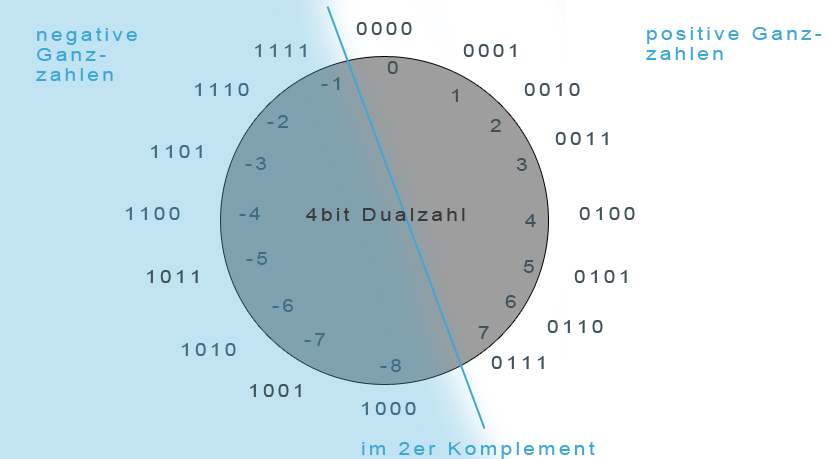
\includegraphics[width=\linewidth]{zahlenkreis_int3.jpg} % Figure image
    \caption{Überlauf mit Integerzahlen } % Figure caption
    % TODO: Ref: https://de.wikipedia.org/wiki/Integer_(Datentyp)#/media/Datei:Zahlenkreis_sint3.jpg
    \label{zahlenkreis} % Label for referencing with \ref{scylla_ring}
\end{figure}


Dadurch führt z.B. beim Datentyp \texttt{int} der Ausdruck \texttt{Integer.MAX\_VALUE + 1} zum Wert \texttt{Integer.MIN\_VALUE}.
Dies kann dazu führen, dass mit \glqq falschen\grqq \ Werten gerechnet wird, ohne dass der Entwickler dies bemerkt.

\subsection{Fliesskommazahlen}
% TODO: Zweierkomplement oben noch nicht beschrieben
Im Gegensatz zur Darstellung im Zweierkomplement, welche für Integer-Typen in Java verwendet werden, werden Fliesskommazahlen intern nach IEEE Standard dargestellt.
Anders als bei der Zweierkomplement-Darstellung sieht dieses Format spezielle Werte für \texttt{POSITIVE\_INFINITY} und \texttt{NEGATIVE\_INFINITY} vor.
%  Quelle: https://stackoverflow.com/questions/41312477/purpose-of-defining-positive-infinity-negative-infinity-nan-constants-only-for

\section{Designentscheidungen}
\subsection{Spezifiziertes Verhalten}
Der neue Datentyp \texttt{nat64} unterstützt die bestehenden Operationen aus IML\footnote{Aktuell sind dies \begin{itemize} \item MULTOPR(*, divE, modE) \item ADDOPR(+, -) \item RELOPR(<, <=, >, >=, =, /=) \item BOOLOPR(/\textbackslash? \textbackslash/?)\end{itemize}}.
Sofern sich die einzelnen Operanden und auch das Resulat im Wertebereich ($\in \mathbb{N}$) befinden, %TODO: + länge max 64-bit
entspricht das Verhalten vom Datentyp \texttt{nat64} jenem vom Datentyp \texttt{int64}.
Andernfalls wird folgendes Verhalten festgelegt:

\begin{itemize} % TODO: Effektives Verhalten anpassen gemäss Entscheidung
    \item \textbf{Wertebereich}: Bei einem Überlauf wird jeweils mit dem maximalen Wert weitergerechnet. Dieser entspricht dem maximalen Wert von \texttt{int64}\footnote{9,223,372,036,854,775,807}.
    \item \textbf{Negative Werte}: Werte werden jeweils als absolute Werte Betrachtet. Ein negativer Wert $-5$ entspricht beispielsweise dem Betrag, also $|-5| = 5$.
    \item \textbf{Rest bei Division}: Wird analog \texttt{int64} behandelt und Nachkommastellen werden abgeschnitten.
\end{itemize}

\subsection{Alternative Ansätze}

% TODO: Downsides z.B. gemäss %  Quelle: https://stackoverflow.com/questions/41312477/purpose-of-defining-positive-infinity-negative-infinity-nan-constants-only-for

\section{Beispielprogramme}
\label{sec:prog}
Operation:
\begin{lstlisting}
program progAddition
global
    var x:nat64;
    var y:nat64;
    var r:nat64;
    var b:bool
do
    x init := 4;
    y init := 3;
    r init := x + y;
    b init := r = 7;

    debugout r;
    debugout b
endprogram
\end{lstlisting}
Casting:
\begin{lstlisting}
program progCasting
global
    var x:nat64;
    var y:int64;
    var r:nat64;
    var b:bool
do
    x init := 4;
    y init := 3;
    r init := x + [nat64] y;
    b init := r = 7;

    debugout r;
    debugout b
endprogram
\end{lstlisting}

%----------------------------------------------------------------------------------------
%	BIBLIOGRAPHY
%----------------------------------------------------------------------------------------

\begin{thebibliography}{9}
	\bibitem{wikipedia}
	Wikipedia: Natürliche Zahl,
	\url{https://de.wikipedia.org/wiki/Nat\%C3\%BCrliche_Zahl}

    \bibitem{wikipedia}
    Wikipedia: Natural numbers (engl.),
    \url{https://en.wikipedia.org/wiki/Natural_number}


\end{thebibliography}
%----------------------------------------------------------------------------------------

\end{document}
